\chapter{Solution Methodology}
\label{sec:methodology}

Having formulated the bilevel knapsack-scheduling problem in Chapter~\ref{sec:formulation}, we now develop solution methods to find optimal or near-optimal solutions efficiently. We begin by discussing a baseline approach based on complete enumeration, which provides a reference for understanding the computational challenges. We then present our main contribution: a branch-and-bound algorithm that systematically explores the search space while using tight upper bounds to prune branches that cannot contain optimal solutions. The key components---branching rules, upper bound computation via a knapsack scheduling relaxation, and efficient dynamic programming for the bounding subproblem---are developed in detail throughout this chapter.

\section{Complete Enumeration (Baseline)}

\subsection{Algorithm}

The most straightforward approach is to enumerate all feasible selections and solve the follower's problem for each:

\begin{algorithm}
\caption{Complete Enumeration for Bilevel Problem}
\label{alg:enumeration}
\begin{algorithmic}[1]
\State $C_{\max}^* \gets 0$, $x^* \gets \emptyset$
\For{each feasible selection $x$ satisfying budget constraint}
    \State Solve follower's scheduling problem to get $C_{\max}(x)$
    \If{$C_{\max}(x) > C_{\max}^*$}
        \State $C_{\max}^* \gets C_{\max}(x)$
        \State $x^* \gets x$
    \EndIf
\EndFor
\State \Return $(x^*, C_{\max}^*)$
\end{algorithmic}
\end{algorithm}

\subsection{Complexity Analysis}

The search space grows exponentially:
\begin{itemize}
    \item Maximum copies of item $i$: $\lfloor B/p_i \rfloor$
    \item Total combinations: $\prod_{i=1}^{n} (\lfloor B/p_i \rfloor + 1)$
    \item For each combination: Check budget constraint and solve scheduling problem after, which in itself is NP-hard.
\end{itemize}

\textbf{Example:} With $n=10$ items, budget $B=100$, and prices $p_i \in [5, 15]$:
\begin{itemize}
    \item Search space $\approx 10^{10}$ to $10^{12}$ combinations
    \item At 1ms per scheduling solve: 115 days to 31 years
    \item Clearly intractable for practical instances
\end{itemize}

\section{Branch-and-Bound Algorithm}

\subsection{Overview}
To overcome the combinatorial explosion of complete enumeration, we develop a branch-and-bound algorithm.
The Branch-and-bound algorithm systematically explores the search space while pruning branches that cannot contain optimal solutions.
Here, all possible selections are organized in a search tree, where each node represents a partial selection of items and each leaf node represents a complete selection.
The algorithm consists of three main components:

\begin{enumerate}
    \item \textbf{Branching:} We decompose the problem into subproblems
    \item \textbf{Bounding:} We compute an upper bound on the best possible solution in a subtree
    \item \textbf{Pruning:} We eliminate subtrees that cannot improve the incumbent
\end{enumerate}

\subsection{Search Tree Structure}

\textbf{Node representation:} Each node represents a partial solution and holds all of the following information:
\begin{itemize}
    \item \textbf{Depth $d$:} All items $1, \ldots, d$ have fixed quantities.
    \item \textbf{Occurrences:} $x = [x_1, \ldots, x_d, ?, \ldots, ?]$
    \item \textbf{Remaining budget:} $B - \sum_{i=1}^{d} p_i x_i$
\end{itemize}

\textbf{Branching rule:} From depth $d$, create children by setting $x_{d+1}$:
\begin{itemize}
    \item Branch for $x_{d+1} = 0, 1, 2, \ldots, \lfloor B_{\text{rem}} / p_{d+1} \rfloor$
\end{itemize}

\textbf{Example search tree:}
Figure~\ref{fig:search-tree} illustrates the branching structure for a problem with 2 items, prices $p_1 = 5$, $p_2 = 8$, and budget $B = 10$.

\begin{figure}[htbp]
\centering
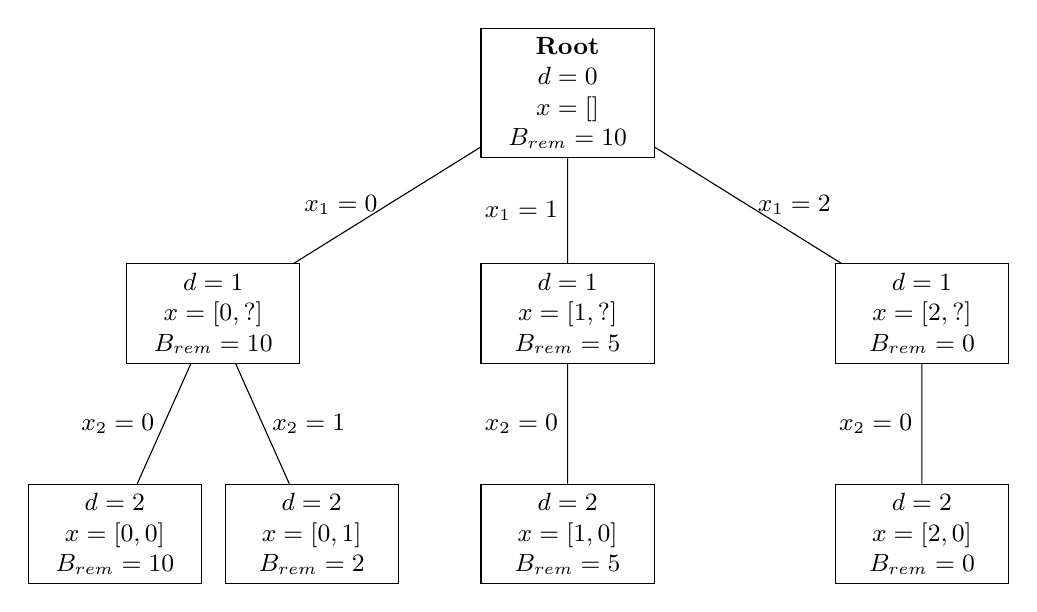
\begin{tikzpicture}[
  level distance=2.8cm,
  level 1/.style={sibling distance=4.5cm},
  level 2/.style={sibling distance=2.5cm},
  node/.style={rectangle, draw, align=center, font=\small, minimum width=2.2cm, minimum height=1.2cm}
]

% Root node
\node[node] (root) {\textbf{Root}\\$d=0$\\$x=[]$\\$B_{\text{rem}}=10$}
  child {node[node] (n1) {$d=1$\\$x=[0,?]$\\$B_{\text{rem}}=10$}
    child {node[node] {$d=2$\\$x=[0,0]$\\$B_{\text{rem}}=10$}
      edge from parent node[left] {\small $x_2=0$}}
    child {node[node] {$d=2$\\$x=[0,1]$\\$B_{\text{rem}}=2$}
      edge from parent node[right] {\small $x_2=1$}}
    edge from parent node[left] {\small $x_1=0$}
  }
  child {node[node] (n2) {$d=1$\\$x=[1,?]$\\$B_{\text{rem}}=5$}
    child {node[node] {$d=2$\\$x=[1,0]$\\$B_{\text{rem}}=5$}
      edge from parent node[left] {\small $x_2=0$}}
    edge from parent node[left] {\small $x_1=1$}
  }
  child {node[node] (n3) {$d=1$\\$x=[2,?]$\\$B_{\text{rem}}=0$}
    child {node[node] {$d=2$\\$x=[2,0]$\\$B_{\text{rem}}=0$}
      edge from parent node[left] {\small $x_2=0$}}
    edge from parent node[right] {\small $x_1=2$}
  };

\end{tikzpicture}
\caption{Example search tree with 2 items ($p_1=5, p_2=8, B=10$). Each node stores depth $d$, partial solution $x$, and remaining budget $B_{\text{rem}}$. Leaf nodes represent complete solutions.}
\label{fig:search-tree}
\end{figure}

\subsection{Upper Bound Computation}

\textbf{Key idea:} In the branch-and-bound tree we systematically explore the search space to find the combination of items that maximizes the result of the follower's problem. Given an incumbent solution with makespan $C_{\max}^{\text{incumbent}}$, we don't want to explore subtrees that cannot yield a better solution. 

At a given subtree rooted at depth $d$, we have already fixed the quantities of item types $1, \ldots, d$. If we can compute an upper bound $\text{UB}(x_1, \ldots, x_d, B_{\text{rem}})$ on the best possible makespan achievable by completing the selection with item types $d+1, \ldots, n$, we can prune the subtree if this upper bound is less than or equal to the incumbent. This follows because no solution in this subtree can improve upon the incumbent and is known in the literature as \emph{bound dominance}.

Formally, since any complete solution satisfies
\begin{equation}
\max_{\substack{x_{d+1}, \ldots, x_n \\ \sum_{i=d+1}^{n} p_i x_i \leq B_{\text{rem}}}} C_{\max}^*(x_1, \ldots, x_d, x_{d+1}, \ldots, x_n) \leq \text{UB}(x_1, \ldots, x_d, B_{\text{rem}}),
\end{equation}
we can safely prune the subtree whenever
\begin{equation}
\text{UB}(x_1, \ldots, x_d, B_{\text{rem}}) \leq C_{\max}^{\text{incumbent}}.
\end{equation}

\textbf{Computing the upper bound:}
The key challenge is to efficiently compute a tight upper bound $\text{UB}(x_1, \ldots, x_d, B_{\text{rem}})$ that overestimates the best possible makespan in the subtree without solving the full bilevel problem. We achieve this by decomposing the bound into two components: the contribution from already-fixed items $1, \ldots, d$, and an optimistic estimate of the contribution from the remaining items $d+1, \ldots, n$.

For the fixed items, we schedule the jobs of types $1, \ldots, d$ with quantities $x_1, \ldots, x_d$ using the Longest-Processing-Time (LPT) rule to obtain makespan $C_{\max}^{\text{LPT},(d)}$. For the remaining items, rather than enumerating all possible selections, we formulate a relaxation that maximizes the additional makespan contribution subject to the remaining budget. This leads to the following optimization problem:

\textbf{Knapsack Scheduling Relaxation:}
\begin{align}
\text{UB}(x_1, \ldots, x_d, B_{\text{rem}}) = & C_{\max}^{\text{LPT},(d)} + \max_{\substack{y_{d+1}, \ldots, y_n}} \sum_{i=d+1}^{n} d_i \left\lceil \frac{y_i}{m} \right\rceil \label{eq:ub}\\
\text{s.t.} \quad & \sum_{i=d+1}^{n} p_i y_i \leq B_{\text{rem}} \nonumber\\
& y_i \in \mathbb{Z}_+ \quad \forall i > d \nonumber
\end{align}
where $C_{\max}^{\text{LPT},(d)}$ denotes the makespan obtained by scheduling jobs of types $1, \ldots, d$ with quantities $x_1, \ldots, x_d$ using the LPT rule, and $y_i$ represents the (to-be-determined) quantity of job type $i$ for items not yet fixed.

The objective function uses the ceiling term $\lceil y_i / m \rceil$ to provide an optimistic estimate over the effect of the item types that still need to be selected.

We now establish that this formulation indeed provides a valid upper bound on the optimal follower makespan for any completion of the partial solution.

\textbf{Validity of the upper bound:}

\begin{theorem}[Upper Bound Validity]
\label{thm:upper-bound}
The upper bound computed by equation~\eqref{eq:ub} is valid, i.e., for any completion of the partial solution $(x_1, \ldots, x_d)$ with items $(x_{d+1}, \ldots, x_n)$, the optimal follower makespan satisfies:
\begin{equation}
C_{\max}^*(x_1, \ldots, x_n) \leq \text{UB}(x_1, \ldots, x_d).
\end{equation}
\end{theorem}

\begin{proof}
We establish the upper bound by analyzing the Longest-Processing-Time (LPT) scheduling rule. Since LPT is a $\frac{4}{3}$-approximation for the $P||C_{\max}$ problem, any upper bound on the LPT makespan provides an upper bound on the optimal makespan.

The Bound is derived as an execution of the LPT rule for the job types $1, \ldots, d$ with quantities $x_1, \ldots, x_d$ and an upper bound on the contribution of the remaining job types $d+1, \ldots, n$ with quantities $y_{d+1}, \ldots, y_n$ chosen to maximize the LPT makespan under the budget constraint.

Consider LPT scheduling on $m$ parallel machines. By construction of the branch-and-bound tree, assume job types are ordered by decreasing processing time: $d_1 \geq d_2 \geq \cdots \geq d_n$. The LPT rule assigns each job to the currently least-loaded machine.

At depth $d$ in the search tree, quantities $x_1, \ldots, x_d$ are fixed, and all copies of these job types have been scheduled using LPT. Let $C_{\max}^{\text{LPT},(d)}$ denote the makespan after scheduling these jobs. To obtain an upper bound, we assume all machines are filled to exactly $C_{\max}^{\text{LPT},(d)}$—this represents a worst-case scenario that can only increase (never decrease) the final makespan.

Now consider scheduling the remaining job types $d+1, \ldots, n$. When we schedule $x_{d+1}$ copies of type $d+1$ (each with duration $d_{d+1}$), the first copy increases the makespan by $d_{d+1}$. Since all machines have equal load, the makespan increases by $d_{d+1}$ again only after placing copies on all $m$ machines. Therefore, scheduling $x_{d+1}$ copies increases the makespan by
\begin{equation}
\left\lceil \frac{x_{d+1}}{m} \right\rceil \cdot d_{d+1}.
\end{equation}

We apply the same reasoning to each subsequent job type $d+2, \ldots, n$. After scheduling all copies of a job type, we again assume all machines are filled to the current makespan—this assumption only provides a further upper bound and avoids case distinctions.

Thus, the LPT makespan satisfies:
\begin{equation}
C_{\max}^{\text{LPT}} \leq C_{\max}^{\text{LPT},(d)} + \sum_{i=d+1}^{n} \left\lceil \frac{x_i}{m} \right\rceil d_i.
\end{equation}

Now, if we choose variables $x_{d+1}, \ldots, x_n$ to maximize this expression subject to the budget constraint $\sum_{i=d+1}^{n} p_i x_i \leq B_{\text{rem}}$, we obtain the bound in equation~\eqref{eq:ub}. Since LPT provides a $\frac{4}{3}$-approximation and our bound applies to LPT scheduling, it also bounds the optimal follower makespan.
\end{proof}

\subsection{Branch-and-Bound Algorithm}

With the search tree structure, upper bound computation, and pruning conditions established, we can now present the complete branch-and-bound algorithm. Algorithm~\ref{alg:bnb} integrates all components: it systematically explores the search tree, computes upper bounds at each node using the knapsack scheduling relaxation, and prunes branches when the bound indicates that no improvement over the incumbent is possible. The algorithm maintains a queue of unexplored nodes and continues until all promising branches have been exhausted.

\begin{algorithm}
\caption{Branch-and-Bound for Bilevel Problem}
\label{alg:bnb}
\begin{algorithmic}[1]
\State Initialize: $(x^*, C_{\max}^*) \gets$ heuristic solution, queue $Q \gets \{$root node$\}$
\While{$Q \neq \emptyset$}
    \State $x \gets Q.\text{pop}()$ \Comment{Node with partial solution at depth $d$}
    \If{$x$ is complete solution}
        \State Solve follower's problem: $C_{\max}(x)$
        \If{$C_{\max}(x) > C_{\max}^*$}
            \State $C_{\max}^* \gets C_{\max}(x)$, $x^* \gets x$ \Comment{Update incumbent}
        \EndIf
    \Else
        \State Compute $B_{\text{rem}} \gets B - \sum_{i=1}^{d} p_i x_i$ \Comment{Remaining budget}
        \State Compute upper bound: $\text{UB}(x_1, \ldots, x_d, B_{\text{rem}})$
        \If{$\text{UB}(x_1, \ldots, x_d, B_{\text{rem}}) \leq C_{\max}^*$}
            \State \textbf{continue} \Comment{Prune: bound dominated}
        \EndIf
        \State Generate children by branching on next item
        \State Add feasible children to $Q$
    \EndIf
\EndWhile
\State \Return $(x^*, C_{\max}^*)$
\end{algorithmic}
\end{algorithm}

\section{Solving the Bounding Subproblem}

The bounding computation requires solving equation~\eqref{eq:ub}, which is a knapsack problem with a modified objective function. Since the original bilevel knapsack-scheduling problem is already weakly NP-hard, and the bounding subproblem inherits similar computational complexity, solving it at every node of the branch-and-bound tree would be prohibitively expensive. To overcome this bottleneck, we adopt a preprocessing strategy: we solve the bounding subproblem once before the branch-and-bound algorithm starts and store all relevant solutions in a table. During the branch-and-bound traversal, we simply look up precomputed entries from this table in constant time, avoiding redundant computations and significantly accelerating the overall algorithm.

\subsection{Dynamic Programming Approach}

We use dynamic programming to solve the ceiling knapsack problem efficiently:

\textbf{State:} $f[i][b] =$ maximum value using items $1, \ldots, i$ with budget $b$

\textbf{Recurrence:}
\begin{equation}
f[i][b] = \max_{k=0}^{\lfloor b/p_i \rfloor} \left\{ f[i-1][b - k \cdot p_i] + d_i \left\lceil \frac{k}{m} \right\rceil \right\}
\end{equation}

\textbf{Complexity:} $O(nBK)$ where $K = \max_i \lfloor B/p_i \rfloor$

\textbf{Practical Implementation:} In practice, we can use a standard knapsack solver that maximizes the sum of durations. For each item type $i$, we create:
\begin{itemize}
    \item One copy of item $i$ with duration $d_i$ and cost $p_i$ (representing taking $1$ to $m-1$ copies)
    \item Multiple "packages of item type $i$" with cost $m \cdot p_i$ and duration $d_i$ each (representing batches of $m$ items)
\end{itemize}
This transformation allows us to use efficient off-the-shelf knapsack solvers while correctly capturing the ceiling effect in the objective function.

\subsection{Optimization: Reversed Item Order}

To efficiently compute bounds at different depths, we pre-solve the DP table with items in reverse order. This allows us to query ``last $k$ items'' efficiently.

\textbf{Example:} Consider a node at depth $d=2$ where we have decided on items $x_1$ and $x_2$, with remaining budget $B_{\text{rem}} = 50$. To compute the upper bound, we need to solve the knapsack scheduling relaxation over items $\{3, 4, \ldots, n\}$ with budget $B_{\text{rem}}$. Since we preprocessed the DP table with items in reverse order (starting from item $n$ down to item $1$), we can directly look up the entry corresponding to ``items $\{3, \ldots, n\}$ with budget $50$'' in constant time. Specifically, we query $f[n-2][50]$, which gives us the maximum achievable makespan contribution from the remaining items, thus providing the second term in equation~\eqref{eq:ub}.

\section{Follower's Scheduling Algorithm}

To compute the first term $C_{\max}^{\text{LPT},(d)}(x_1, \ldots, x_d)$ in equation~\eqref{eq:ub}, we apply the \textbf{Longest Processing Time (LPT)} rule. This term represents the makespan contribution from the decided items at a given node. 

Since item types are presorted from longest to shortest duration, the algorithm processes jobs in non-ascending order of processing time, greedily assigning each job to the least loaded machine:

\begin{algorithm}
\caption{LPT Scheduling for $C_{\max}^{\text{LPT},(d)}$ Computation}
\label{alg:scheduling}
\begin{algorithmic}[1]
\State Initialize machine loads: $L_1, \ldots, L_m \gets 0$
\For{each job $j$ with duration $d_j$ (in non-ascending order)}
    \State $k^* \gets \arg\min_{k} L_k$ \Comment{Find least loaded machine}
    \State $L_{k^*} \gets L_{k^*} + d_j$ \Comment{Assign job to machine $k^*$}
\EndFor
\State \Return $C_{\max}^{\text{LPT},(d)} = \max_k L_k$
\end{algorithmic}
\end{algorithm}

\textbf{Complexity:} $O(J \log m)$ for $J$ jobs (using a priority queue)

\textbf{Optimality:} The LPT rule is a $\frac{4}{3}$-approximation for makespan minimization, and often produces optimal or near-optimal solutions in practice.

\textbf{Incremental Updates:} Importantly, we do not recompute $C_{\max}^{\text{LPT},(d)}$ from scratch at each node. Instead, when generating a child node by deciding on item type $d+1$ with quantity $x_{d+1}$, we incrementally update the machine loads by adding the $x_{d+1}$ jobs of duration $d_{d+1}$ to the current schedule. Similarly, the remaining budget $B_{\text{rem}}$ is updated incrementally by subtracting $p_{d+1} \cdot x_{d+1}$ from the parent node's remaining budget. This incremental approach significantly reduces computational overhead during tree traversal.

\section{Another Upper Bound: Maximizing the LPT Rule}

While the branch-and-bound algorithm uses the LPT rule to model the follower's scheduling behavior, we can exploit this connection to derive tighter bounds and better initial solutions. Since maximizing the LPT makespan provides a provably good approximation to the leader's optimal solution, we can use this approach in two ways: first, solving the Max-LPT problem before starting the branch-and-bound algorithm yields a strong initial incumbent; second, applying the Max-LPT approach at each node in the search tree provides an alternative upper bound for pruning. We will compare the computational trade-offs between different bounding strategies experimentally in Chapter~\ref{sec:experiments}.

\subsection{The Max-LPT Problem}

Recall that the \textbf{Longest Processing Time (LPT) rule} schedules jobs in decreasing order of their processing times, always assigning the next job to the machine with the smallest current load. This greedy rule is well-known to provide good makespan approximations for parallel machine scheduling.

We now define the \textbf{Max-LPT problem} as follows:

\begin{definition}[Max-LPT Problem]
Given item types $1, \ldots, n$ with durations $d_i$ and costs $p_i$, a number of machines $m$, and a budget constraint $B$, the Max-LPT problem seeks to find a combination of items $(x_1, \ldots, x_n)$ with $x_i \geq 0$ (allowing multiple copies of each item type) such that:
\begin{itemize}
    \item The budget constraint is satisfied: $\sum_{i=1}^{n} p_i x_i \leq B$
    \item The makespan is maximized when the selected jobs are distributed on the machines using the LPT rule
\end{itemize}
\end{definition}

In other words, the Max-LPT problem asks: what is the best job selection that maximizes the makespan achievable by the LPT scheduling rule?

\subsection{Approximation Guarantee}

Before presenting the algorithm for solving the Max-LPT problem, we establish its connection to the original knapsack-scheduling problem.

\begin{theorem}[3/4-Approximation Guarantee]
\label{thm:maxlpt-approx}
Let $C_{\max}^{\text{LPT}}$ denote the optimal value of the Max-LPT problem, and let $C_{\max}^{\text{OPT}}$ denote the optimal value of the knapsack-scheduling problem (with optimal scheduling). Then
\[
C_{\max}^{\text{LPT}} \geq \frac{3}{4} \cdot C_{\max}^{\text{OPT}}.
\]
\end{theorem}

To prove this result, we first establish two general results about approximation algorithms and their application to bilevel optimization problems.

\begin{lemma}[Properties of approximation algorithms]
\label{lem:approx-properties}
Let \texttt{approx} be an approximation algorithm for a minimization problem with approximation constant $\alpha \ge 1$. Then there exists a constant $\beta := \frac{1}{\alpha}$ such that
\[
\beta \cdot \mathrm{Opt} \le \beta \cdot \mathrm{approx} \le \mathrm{Opt} \le \mathrm{approx}.
\]
\end{lemma}

\begin{proof}
Since \texttt{approx} is an approximation algorithm for a minimization problem with approximation constant $\alpha$, it holds that
\[
\mathrm{Opt} \le \mathrm{approx} \le \alpha \cdot \mathrm{Opt}.
\]
Setting $\beta = \frac{1}{\alpha}$ and multiplying both sides by $\beta$, we obtain
\[
\beta \cdot \mathrm{Opt} \le \beta \cdot \mathrm{approx} \le \mathrm{Opt} \le \mathrm{approx}.
\]
which proves the claim.
\end{proof}

\begin{theorem}[Approximation algorithms and bilevel optimization problems]
\label{thm:approx-bilevel}
Let a bilevel optimization problem $\max_{x \in \mathcal{X}} \min_{y \in \mathcal{L}(x)} c\bigl(x, y\bigr)$ be given and let $\mathrm{approx}$
be a function such that there exists a constant $\beta \le 1$ fulfilling:
\begin{enumerate}
    \item $\mathrm{approx}(x) \in \mathcal{L}(x)$ for all $x \in \mathcal{X}$,
    \item $
    \beta \cdot c\bigl(x, y^*(x)\bigr)\le \beta \cdot c\bigl(x, \mathrm{approx}(x)\bigr) \le c\bigl(x, y^*(x)\bigr) \le c\bigl(x, \mathrm{approx}(x)\bigr) $
\end{enumerate}
where $y^*(x)$ denotes an optimal lower-level solution for fixed $x$.

If $
\hat{x} \in \arg\max_{x \in \mathcal{X}} c\bigl(x, \mathrm{approx}(x)\bigr),$
then it follows that
\[
\beta \cdot \mathrm{Opt} \le c\bigl(\hat{x}, y^*(\hat{x})\bigr) \le \mathrm{Opt},
\]
i.e., $c\bigl(\hat{x}, y^*(\hat{x})\bigr)$ is a $\beta$-approximate solution of the bilevel problem $\max_{x \in \mathcal{X}} \min_{y \in \mathcal{L}(x)} c\bigl(x, y\bigr)$.
\end{theorem}

\begin{proof}
By definition of $\hat{x}$ we have
\[
c\bigl(\hat{x}, \mathrm{approx}(\hat{x})\bigr)
\;\ge\;
c\bigl(x^*, \mathrm{approx}(x^*)\bigr),
\]
where $x^*$ is an optimal upper-level solution.

Putting everything together, we obtain
\[
c\bigl(\hat{x}, y^*(\hat{x})\bigr)
\;\ge\;
\beta \cdot c\bigl(\hat{x}, \mathrm{approx}(\hat{x})\bigr)
\;\ge\;
\beta \cdot c\bigl(x^*, \mathrm{approx}(x^*)\bigr)
\;\ge\;
\beta \cdot c\bigl(x^*, y^*(x^*)\bigr)
=
\beta \cdot \mathrm{Opt}.
\]
This proves the claim.
\end{proof}

\begin{proof}[Proof of Theorem~\ref{thm:maxlpt-approx}]
We apply Theorem~\ref{thm:approx-bilevel} to our knapsack-scheduling problem. The LPT rule is known to be a $\frac{4}{3}$-approximation algorithm for the makespan minimization problem on parallel machines. 
By Lemma~\ref{lem:approx-properties}, this means that for any job selection $x$ and $\beta = \frac{3}{4}$, we get:

\[
\frac{3}{4} \cdot \mathrm{Opt} \le \frac{3}{4} \cdot C_{\max}^{\text{LPT}}(\hat{x}) \le \mathrm{Opt} \le C_{\max}^{\text{LPT}}(\hat{x})
\]

By that, we fulfill the conditions of Theorem~\ref{thm:approx-bilevel}.

Now, let $\hat{x}$ be the solution that maximizes the LPT makespan, i.e., $\hat{x}$ solves the Max-LPT problem. Applying Theorem~\ref{thm:approx-bilevel} with $\beta = \frac{3}{4}$, we obtain:
\begin{equation*}
\frac{3}{4} \cdot C_{\max}^{\text{OPT}} \leq C_{\max}^{\text{OPT}}(\hat{x}) \leq C_{\max}^{\text{OPT}}.
\end{equation*}
Since $\hat{x}$ maximizes the LPT makespan, we have $C_{\max}^{\text{LPT}} = C_{\max}^{\text{LPT}}(\hat{x})$, and therefore:
\begin{equation*}
C_{\max}^{\text{LPT}} \geq \frac{3}{4} \cdot C_{\max}^{\text{OPT}}.
\end{equation*}
\end{proof}

This result is significant because it guarantees that solving the Max-LPT problem provides a constant-factor approximation for the harder problem of finding the optimal job selection under optimal scheduling. Moreover, as we will show next, the Max-LPT problem can be solved optimally in pseudo-polynomial time.

\subsection{Ordered Makespan Notation}

Before presenting the algorithm, we introduce notation for the ordered machine loads in a schedule. Given a schedule that assigns jobs to $m$ machines, let $L_1, L_2, \ldots, L_m$ denote the total processing times (loads) on each machine. We define the \textbf{ordered makespan sequence} as follows:

\begin{definition}[Ordered Makespan]
For a given schedule on $m$ machines, let $L_1, L_2, \ldots, L_m$ denote the machine loads. We define:
\begin{itemize}
    \item $C_{\max}^{(1)}$ is the \textbf{standard makespan}, i.e., the maximum load over all machines:
    \[
    C_{\max}^{(1)} = \max_{k=1,\ldots,m} L_k
    \]
    \item $C_{\max}^{(2)}$ is the \textbf{second-largest} machine load:
    \[
    C_{\max}^{(2)} = \max_{k=1,\ldots,m} \left\{ L_k \mid L_k < C_{\max}^{(1)} \right\}
    \]
    \item More generally, $C_{\max}^{(i)}$ is the $i$-th largest machine load for $i = 1, 2, \ldots, m$
    \item $C_{\max}^{(m)}$ is the \textbf{minimum} machine load:
    \[
    C_{\max}^{(m)} = \min_{k=1,\ldots,m} L_k
    \]
\end{itemize}
\end{definition}

In other words, if we sort the machine loads in decreasing order as $L_{\sigma(1)} \geq L_{\sigma(2)} \geq \cdots \geq L_{\sigma(m)}$ for some permutation $\sigma$, then $C_{\max}^{(i)} = L_{\sigma(i)}$ for $i = 1, \ldots, m$. This notation allows us to refer to machines by their relative load ordering rather than their indices.

\subsection{Algorithm Description and Correctness}

The Key observation is that in an optimal solution, the last job i that was scheduled either changed the makespan or it did not. If it did, we know that the last job i was put on the machine corresponding to $C_{\max}^{(m)}$ and since we have an optimal solution, there cannot be a combination of jobs so that the LPT rule would deliver a larger $C_{\max}^{(m)}$ given the budget $B - c_i$.
If the last job that was scheduled did not change the makespan, we know that there has to be another job j that was scheduled earlier and the combination of jobs before the job j maximizes the $C_{\max}^{(m)}$ at the time j was placed. All jobs that are scheduled after j do not chnage the makespan by our assumption. We use this observation to solve the max-LPT problem:
By considering all item types as candidates for the last job and optimizing the preceding schedule accordingly, we can find the optimal solution to the max-LPT problem.

\begin{theorem}
The following algorithm always computes an optimal solution for the \textsc{Max-LPT} problem.
\end{theorem}

\begin{algorithm}[H]
\caption{\textsc{Max-LPT}}
\label{alg:maxLPT}
\begin{algorithmic}[1]
\Require Budget $B$, item types ${ 1\dots, n}$, number of machines $m$
\Ensure Optimal value for the Max-LPT problem

\State Precompute the DP table $DP(i,b)$ for the unbounded knapsack problem
\State Initialize incumbent $z^* \gets 0$
\State Compute $B_i := \left\lfloor \frac{B}{m} \right\rfloor$
\State $\hat{B} := B - m \cdot B_i$

\For{each item $i \in {1,\ldots,n}$}
    \If{$\hat{B} > i.\text{cost}$}
        \State $k \gets 0$
        \While{$\hat{B} > c_i$}
            \State $k \gets k + 1$
            \State Compute $B_i := \left\lfloor \frac{B - k \cdot m}{m} \right\rfloor$
            \State $\hat{B} := B - m \cdot B_i$
        \EndWhile
        \State $z \gets$ DP$(i, B_i) + d_i$
        \If{$z > z^*$}
            \State $z^* \gets z$     
    \EndIf
    \Else
        \State $z \gets$ DP$(i, B_i) + d_i$
        \If{$z > z^*$}
            \State $z^* \gets z$     
        \EndIf
    \EndIf
\EndFor

\State \Return $z^*$
\end{algorithmic}
\end{algorithm}

\paragraph{Running time.}
The running time of the algorithm is
\[
\mathcal{O}(n \cdot B).
\]

\subsection{Correctness Proof}

\begin{proof}
We begin with the key observation:

In an optimal solution of the max-LPT problem, the job $I$ that finishes last is assigned to the machine with the shortest total processing time $C_{\max}^{(m)}$ at that moment. Therefore, the makespan is determined by the duration of this final job $d_I$ together with $C_{\max}^{(m)}$ at that moment.
Since we assume to have an optimal solution, there cannot be a combination of jobs so that the LPT rule would deliver a larger $C_{\max}^{(m)}$ for the subproblem without the final job.
We exploit this property by considering each item type $i$ as a candidate for the job that finishes last. For a fixed candidate $i$, we maximize the makespan of the remaining jobs under the remaining budget.

Let
\[
B_i := \left\lfloor \frac{B}{m} \right\rfloor
\]
be the budget that can be allocated to each machine if the total budget is distributed evenly. Let
\[
\hat{B} = B - m \cdot B_i
\]
be the remaining budget.

If $\hat{B} \ge c_i$, the final job of type $i$ can be paid without reducing the per-machine budget. In this case, the optimal combination of jobs scheduled before $i$ is given by the unbounded knapsack solution stored in $DP(i, B_i)$. This corresponds to the "else" clause of the algorithm.

If $\hat{B} < c_i$, the per-machine budget $B_i$ must be reduced uniformly until the remaining budget is sufficiently big enough to pay for item $i$. After this adjustment, the optimal combination of jobs scheduled before $i$ is again obtained from the dynamic programming table $DP(i, B_i)$. This corresponds to the "if" clause of the algorithm.

Since the algorithm evaluates all item types as possible final jobs and, for each of them, computes the optimal preceding schedule, it considers all candidates for an optimal solution. By selecting the maximum makespan among these candidates, the algorithm returns an optimal solution to the max-LPT problem.
\end{proof}

\subsection{Connection to Knapsack-Scheduling Problem}

The max-LPT algorithm provides a good approximation to the leader's problem by maximizing the makespan under the LPT scheduling rule. While the LPT rule is itself an approximation for optimal scheduling, this algorithm finds the \emph{optimal} job selection that maximizes the LPT makespan. 
We have already shown that this approach yields a $\frac{3}{4}$-approximation for the original knapsack-scheduling problem. If we solve the max-LPT problem before calling the branch and bound Algorithm we use to obtain an optimal solution to the bilevel knapsack-scheduling problem, we obtain a starting incumbent that is guaranteed to be within $\frac{3}{4}$ of the optimal solution. 
In the branch and bound algorithm itself, we can use the max-LPT algorithm to compute upper bounds at each node by evaluating the max-LPT solution for the remaining budget and item types. This provides an upper bound with a $\frac{3}{4}$-approximation guarantee, which is better than the upper bound we used before. 
The disadvantage of this approach is that we have to compute the unbounded knapsack DP table for each depth d in the branch and bound tree, since the remaining item types change at each depth:
In the max-LPT algorithm, we need to solve the unbounded knapsack problem for the remaining item types $d+1, \ldots, n$ at depth $d$.
Since we have to regard every item type $i \in \{d+1, \ldots, n\}$ as a candidate for the last job that finishes, we need to be able to evaluate the best possible combination of item types $d+1, \ldots, i$ for each budget. 
The unbounded knapsack DP tables computed before start from item type $1$ up to item type $d$ and therefore cannot be used again as we increase the depth in the branch and bound tree.
In total, we have to compute n DP tables, one for each possible depth in the tree. Each DP table requires O((n-d)B) time to compute.
This is computationally more expensive than our previous upper bound, which only required a single DP table computed once before the branch and bound traversal. 
We compare both upper bounds experimentally in Chapter~\ref{sec:experiments} to evaluate the trade-off between tighter bounds and computational overhead.